\chapter{Solution}
\change[inline]{describes misto relate}
\change[inline]{aim at}
The section describes the complete solution to solve the scenarios.
We will start with an overview of the solution's parts.
Then, we will give a detailed description of each part.
\par
\begin{figure}[H]\centering
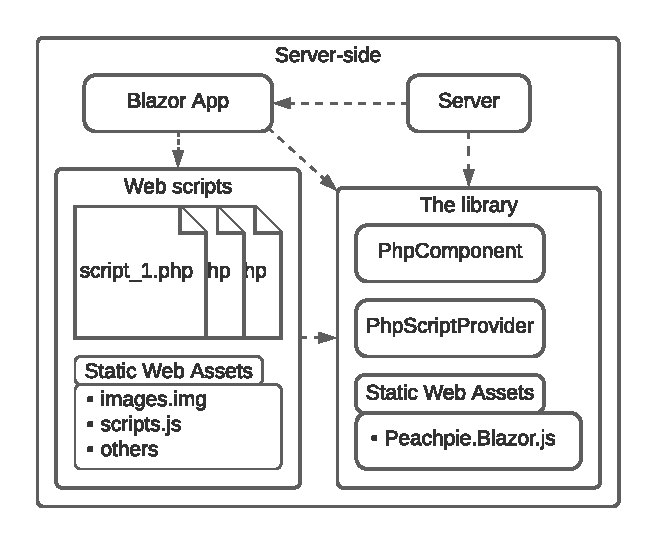
\includegraphics[scale=0.7]{./img/SolutionInfrastructure}
\caption{The solution's infrastructure.}
\label{img03:infrastructure}
\end{figure} 
\par
Figure \ref{img03:infrastructure} illustrates the composition of projects forming a Blazor website, which will use PHP scripts.
There are four projects on the server-side.
We can see the user's defined PHP scripts in the Web scripts project.
Peachpie will compile the project to the .NET assembly.
The next project is a library containing an API for including PHP scripts to the website.
There are PhpComponent and PhpScriptProvider, mentioned earlier, together with additional code support necessary for the correct functionality.
There is the Blazor App project, which becomes the environment for running PHP scripts in a browser.
The server serves these projects.
The server has to provide additional static web assets contained in Web scripts and The library projects.
Dot lines represent references between projects.
We can see the library provides functionality to the server, Blazor App, and the scripts.
Blazor App injects the scripts using the components.
We can see an instance of the Blazor App on the client-side.
Arrows indicate an interaction between the sides. 
\par
The first part will aim at PhpComponent.
It will introduce the implementation problems connected to creating render demanding applications, and it will present the proposed solution.
The second part will talk about PhpScriptProvider.
It will suggest a convenient way how to include the scripts into a browser, and it will present the component's design.
The last part of the description will relate to the server's settings.

\section{PhpComponent}

\change[inline]{Problem struct creation in BuildRenderTree}
\change[inline]{PhpComponent structure}
\change[inline]{Additional API for tag, attributes, + rendering + timer}
\change[inline]{Javascript interop}

\section{PhpScriptProvider}

\change[inline]{Division into functionalities (Router, ScriptProvider, Script)}
\change[inline]{Common things(Script finding,rendering, context, Context save, Using forms, files, parsing url)}
\change[inline]{Router navigating}
\change[inline]{ScriptProvider navigating}
\change[inline]{Script navigating}

\section{Server}
\change[inline]{serving web static assets}